\documentclass[10pt,conference,compsocconf]{IEEEtran}

\usepackage{hyperref}
\usepackage{graphicx}
\usepackage{xcolor}
\usepackage{blindtext, amsmath, comment, subfig, epsfig }
\usepackage{caption}
\usepackage{algorithmic}
\usepackage{cite}
\usepackage[utf8]{inputenc}
\usepackage{csquotes}


\title{CS523 Project 1 Report}
\author{Elvric Trombert, Author 2}
\date{February 2020}

\begin{document}

\maketitle

\begin{abstract}
    Please report your design, implementation details, findings of the first project in this report. \\
    You can add references if necessary. \\
    THE REPORT SHOULD NOT EXCEED 2 PAGES.
\end{abstract}

\section{Introduction}
Secure Multiparty Computation as described by \cite[Frikken]{Frikken2011} \enquote{allow for the distributed computation of a
function over distributed inputs without revealing additional information about the inputs.}

In this project we have implemented an instance of SMC using a Trusted Third party to share secret shares and final
computation of functions.

\section{Threat model}
In SMC the main goal of the adversary is to gain knowledge of the inputs used by the system in the computation of
the function.

This model protects against \textit{passive but curious} adversaries.
In this model the adversary is only capable of passively listening to the information transitioning between a server and
parties and cannot deviate from the protocol.

The adversary is only able to know the secrets of parties it controls, and the result of the function computed.

Depending on the type of function and number of parties the adversary could infer some information such as an
upper or lower bound or even the exact values of other parties secret inputs.

\section{Implementation details}
The SMS protocol was implemented using a trusted third party that receives all, but the local secret shares of each party
as well as the result of the computed function by each party.

\section{Performance evaluation}
All measurements were performed directly on each party and recorded.
The bytes in and out where measured on every
network call made by the party.
The runtime was measured as the time elapsed between the start the run function in
party\_smc.py and the time when that function returns.
Every individual case in each condition was run a total of 10 times.
Unless otherwise specified the number of parties involved in each test was 5.
The standard error calculated as $\frac{\sigma}{\sqrt{n}}$ where n is the number of data entries for each case.
However, in certain graphs that error was way too small relative to the scale to be visible.
The hardware used to run the test was on an i7 UX433F Asus Zenbook.



\begin{figure}[ht]
    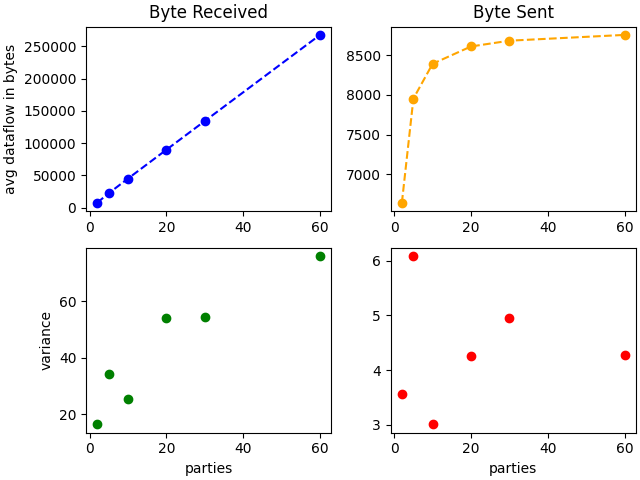
\includegraphics[width=0.49\linewidth]{../performance_analysis/dataflow_num_party_change.png}
    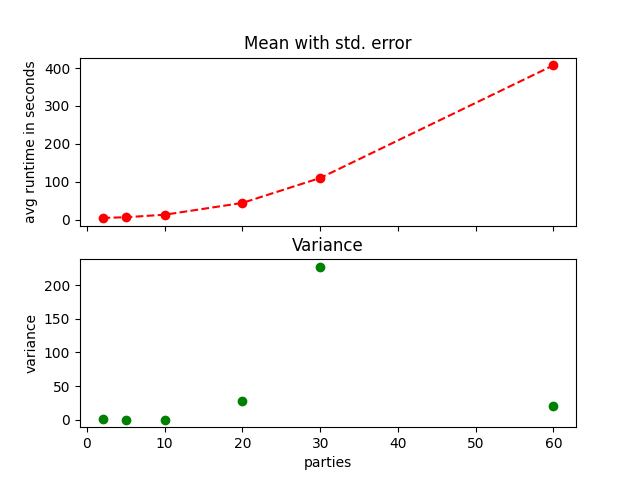
\includegraphics[width=0.49\linewidth]{../performance_analysis/runtime_num_party_change.png}
    \caption{Avg Runtime and Dataflow change based on the number of parties}
    \label{fig:num_parties}
\end{figure}


\begin{figure}[ht]
    \centering
    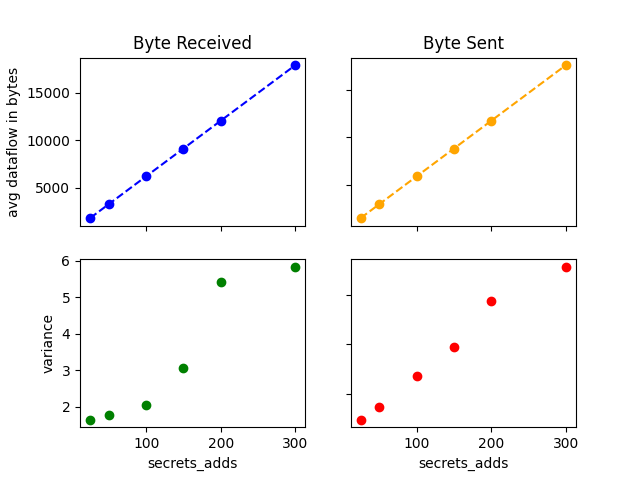
\includegraphics[width=0.49\linewidth]{../performance_analysis/dataflow_secrets_additions.png}
    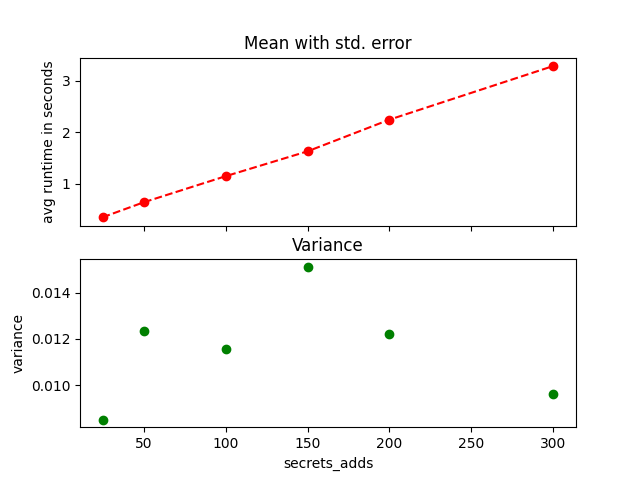
\includegraphics[width=0.49\linewidth]{../performance_analysis/runtime_secrets_additions.png}
    \caption{Avg Runtime and Dataflow change based on the number of Secret Addtions}
    \label{fig:num_additions}
\end{figure}

\begin{figure}[h!]
    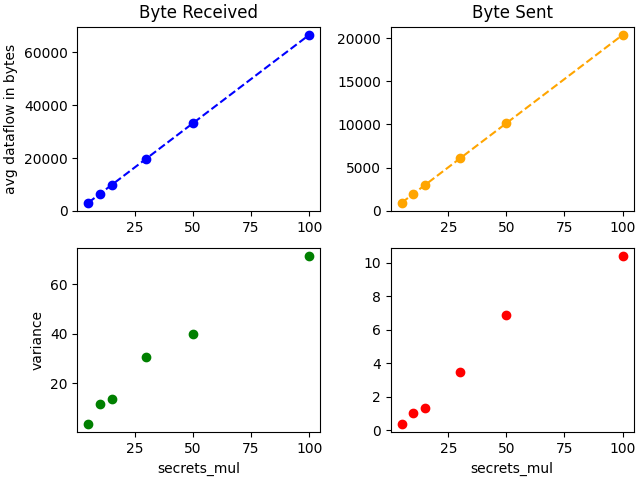
\includegraphics[width=0.49\linewidth]{../performance_analysis/dataflow_secrets_multiplications.png}
    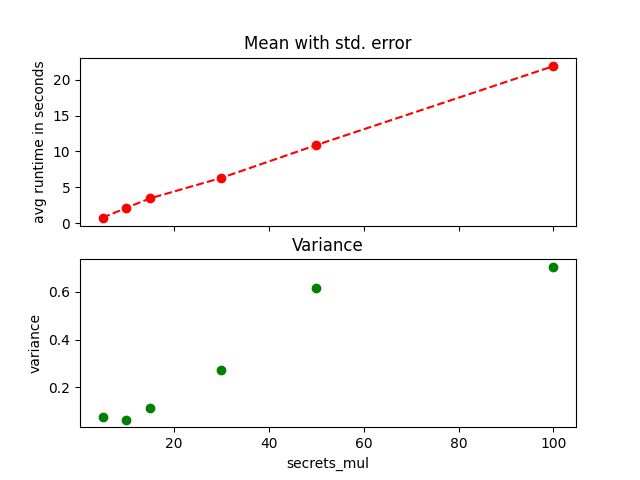
\includegraphics[width=0.49\linewidth]{../performance_analysis/runtime_secrets_multiplications.png}
    \caption{Avg Runtime and Dataflow change based on the number of Secret Multiplications}
    \label{fig:num_multiplications}
\end{figure}

\begin{figure}[h!]
    \centering
    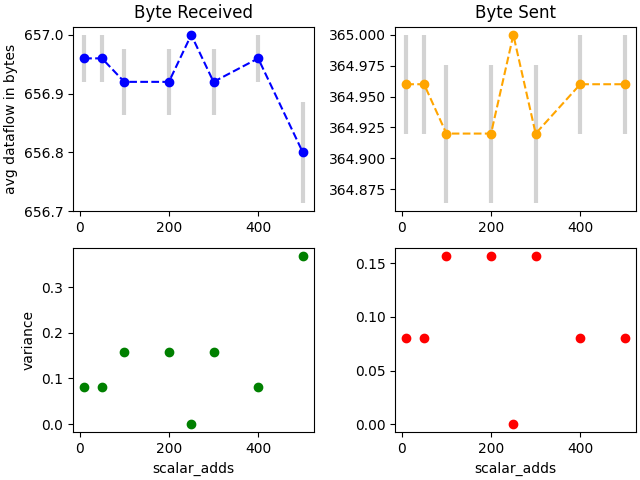
\includegraphics[width=0.49\linewidth]{../performance_analysis/dataflow_scalar_additions.png}
    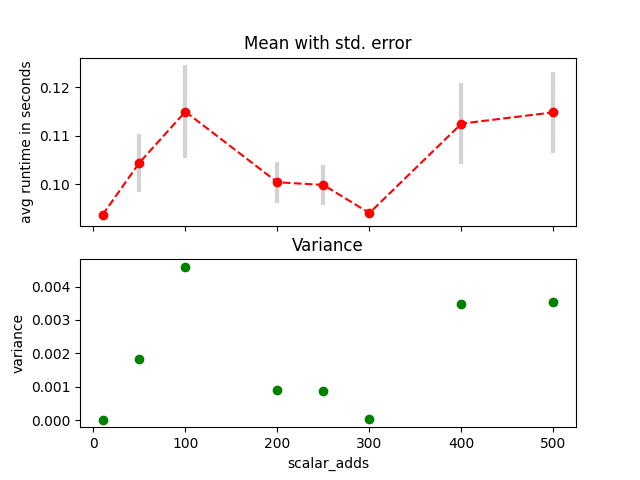
\includegraphics[width=0.49\linewidth]{../performance_analysis/runtime_scalar_additions.png}
    \caption{Avg Runtime and Dataflow change based on the number of Scalar Addtions}
    \label{fig:scalar_add}
\end{figure}


\begin{figure}[h!]
    \centering
    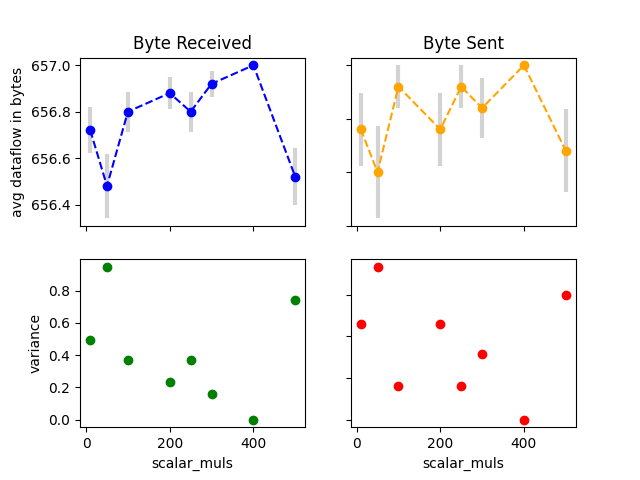
\includegraphics[width=0.49\linewidth]{../performance_analysis/dataflow_scalar_multiplications.png}
    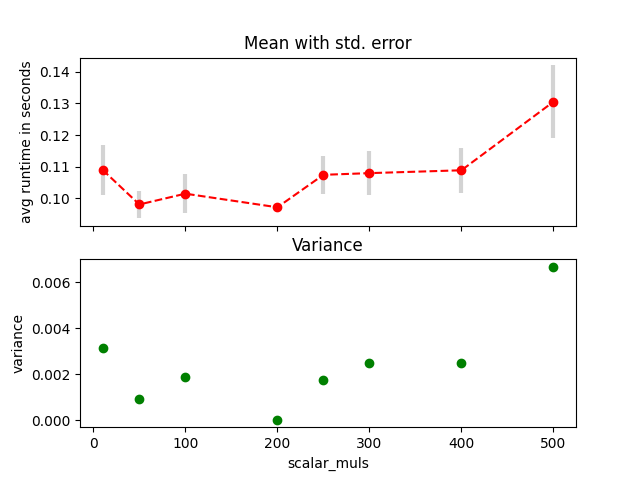
\includegraphics[width=0.49\linewidth]{../performance_analysis/runtime_scalar_multiplications.png}
    \caption{Avg Runtime and Dataflow change based on the number of Scalar Multiplications}
    \label{fig:scalar_mult}
\end{figure}


\subsection{Effect on of the number of parties \ref{fig:num_parties}}
This specific test was run on an expression containing 60 secrets in the form: $s_1 + s_2 + s+_3 \dots s_{30} * s_{31} *
s_{32} * \dots*  s_{60}$

For, the dataflow we can see a linear increase for the number of bytes received, and a logarithmic increase for the
number of bytes sent.
The computational time seems to increase exponentially.
The linear increase in bytes received is expected as every time the number of parties increase by two so does the number
of $x-a$ and $y-b$ input required to perform the secret to secret multiplications since the number of these values to
retrieve are dependent on the number of parties.

The logarithmic increase in bytes sent can be explained by the ration between the number of shares to send vs the
number of parties to send these shares to.
As, the number of secret per party decreases the number of party to send the secret shares to increases counter balancing
the decrease.


\subsection{Effect of number of Secret Additions \ref{fig:num_additions}}

For the dataflow we can see a linear increase in bytes sent and received.
The runtime increases linearly as well.
The variance itself although increasing as the number of addition increases does not go beyond 10.

\subsection{Effect of Number of Secret Multiplication \ref{fig:num_multiplications}}
Both for the dataflow and computation time show a linear increase.

\subsection{Effect of Number of scalars \ref{fig:scalar_add}\ref{fig:scalar_mult}}
For these we see no significant difference in the number of bytes sent and received
which is explained by the fact that scalars are constants and shared across all parties, meaning that no network
IO is required to perform the computation.
The only slight differences shown by the variance and error bars are caused by the serialization of the data.

When it comes to the runtime we can see a slight inconsistent increase.
This is probably due to the fact that since these operations do not require any Network I/O there are more
prone to the CPU computational noise.

\section{Application}
Detail the use case of SMC and a circuit for this use case. Discuss possible privacy leakage not
covered by SMC. Discuss a mitigation if needed.

\bibliographystyle{IEEEtran}
\bibliography{bib}
\end{document}
